\apendice{Documentación de usuario}

\section{Introducción}
En este anexo se va a realizar un manual de usuario detallado en el que se describa el uso de las diferentes características que ofrece el \textit{software} desarrollado de una forma sencilla para que cualquier persona sea capaz de entenderlo y poder utilizar la aplicación con normalidad, reduciendo la curva de aprendizaje que habría si no se tuviese este manual.

\section{Requisitos de usuarios}
Al tratarse de una aplicación web, los requisitos necesitados no son demasiados.
El usuario final de la aplicación tan solo necesita contar con un dispositivo con acceso a internet (en caso de tener la aplicación desplegada en un servidor externo a la red del dispositivo) y un navegador web con JavaScript habilitado.

El \textit{software} desarrollado cuenta con un correcto funcionamiento, al menos, bajo cualquiera de los siguientes navegadores:

\begin{enumerate}
\item Google Chrome (probado bajo la versión 114.0.5735.135)
\item Mozilla Firefox (probado en la versión 114.0.2)
\item Microsoft Edge (probado en la versión 114.0.1823.58)
\item Safari
\item Opera (probado en la versión 100.0.4815.21)
\end{enumerate}

\section{Instalación}
Al tratarse de una aplicación web no precisa de instalación, tan solo se debe acceder a la URL bajo la que se encuentre desplegada la aplicación. 
A la hora de realizar este trabajo, la URL de acceso es \url{https://flask-ubu.herokuapp.com/}

\section{Manual del usuario}
El siguiente manual de usuario se va a realizar con un usuario con permisos de modificación para poder mostrar todas las características de la web.
En caso de contar con un usuario con únicamente permisos de lectura, se mostrará parte de la información que aparece en este manual y otros elementos se encontrarán ocultos.

\subsection{Inicio de sesión}

Para comenzar a utilizar la aplicación lo primero que se debe hacer es acceder a la URL\footnote{A día de realización del trabajo: \url{https://flask-ubu.herokuapp.com/}} de la aplicación.

Al acceder a la dirección de la web por primera vez, se mostrará la página de inicio de sesión (ver figura~\ref{pag:login}) desde donde se debe indica el correo electrónico y la contraseña de la cuenta a utilizar.
La cuenta de correo y la contraseña debe ser la misma que la utilizada en el Moodle de la universidad.

\begin{figure}
	\centering
	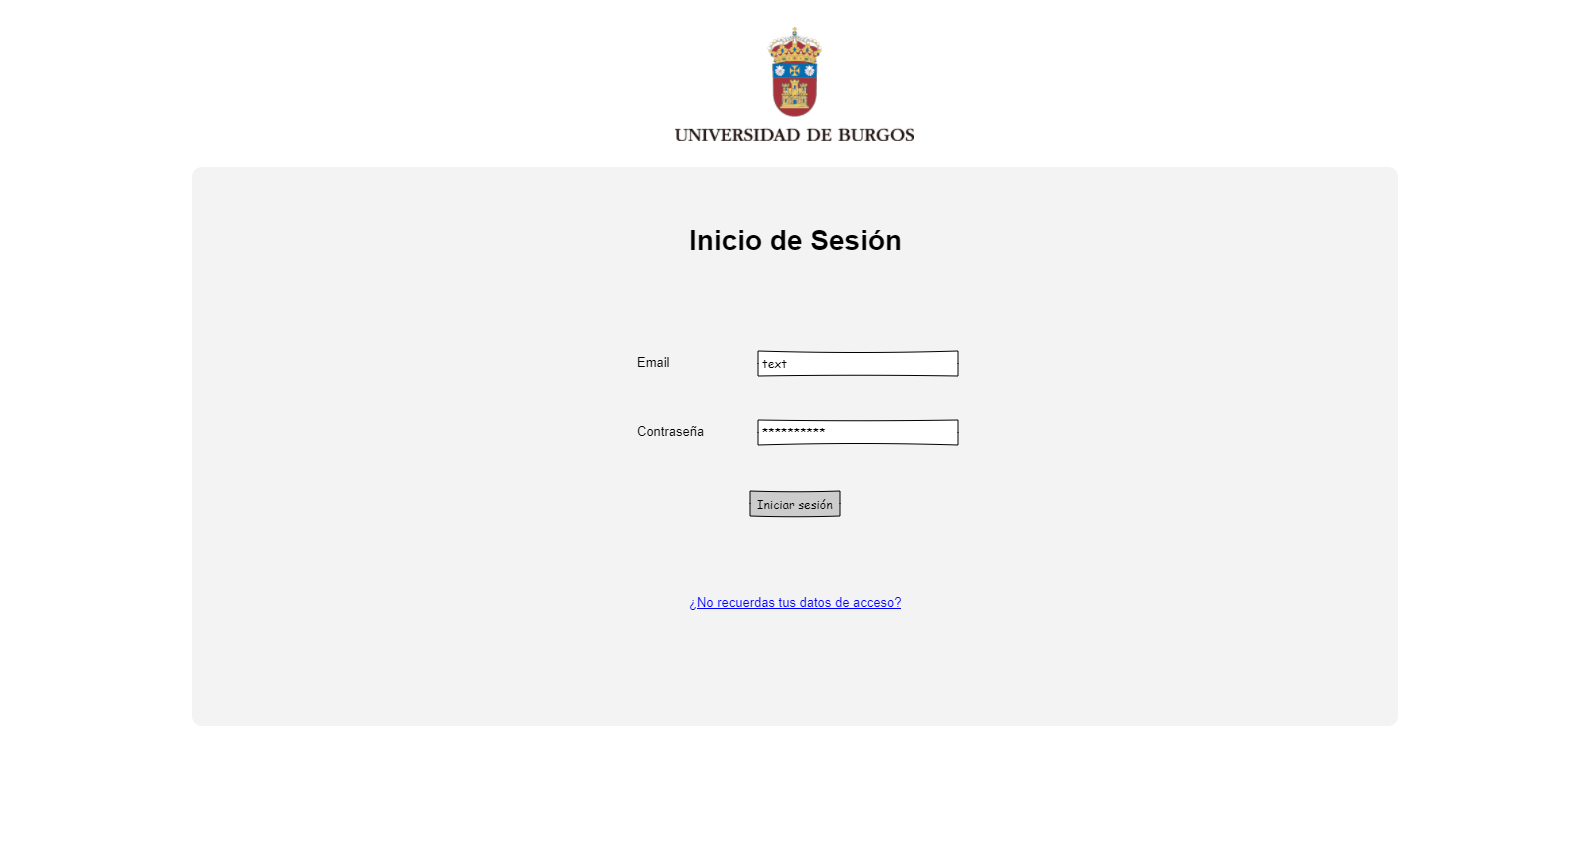
\includegraphics[width=\textwidth]{../img/Anexos/Manual usuario/login.png}
	\caption{Página de inicio de sesión}\label{pag:login}
\end{figure}

Si los datos de acceso son correctos, se tendrá acceso a la aplicación y se mostrará la página principal (imagen~\ref{pag:inicio}).
Una vez se tiene acceso a esta página, se puede acceder al resto de recursos de la web a través del menú superior de navegación.

\begin{figure}
	\centering
	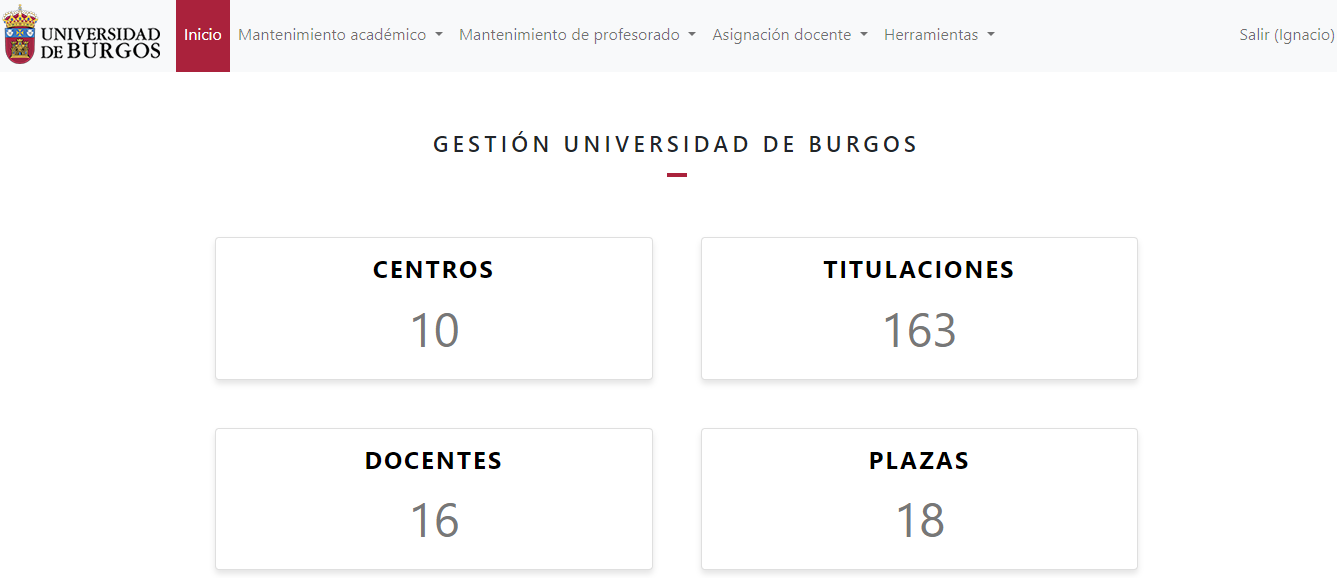
\includegraphics[width=\textwidth]{../img/Anexos/Manual usuario/inicio.png}
	\caption{Página principal}\label{pag:inicio}
\end{figure}

\subsection{Mantenimiento académico}
A continuación se van mostrar las diferentes funcionalidades dentro del mantenimiento académico de la aplicación.
Para ello, se debe pulsar sobre la opción del menú llamada <<Mantenimiento académico>> desde la que se desplegarán las opciones disponibles dentro de esta (imagen~\ref{pag:menuManAc}), las cuales son <<Centros>>, <<Titulaciones>> y <<Asignaturas>>.
Desde cada una de estas opciones se podrá realizar la visualización, creación y actualización de cada uno de estos componentes.

\begin{figure}
	\centering
	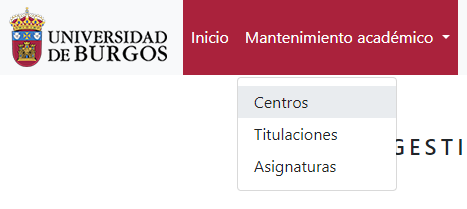
\includegraphics[width=\textwidth]{../img/Anexos/Manual usuario/menu man ac.png}
	\caption{Menú: Mantenimiento académico}\label{pag:menuManAc}
\end{figure}

\subsubsection{Creación de centros}
Pulsando sobre la opción del menú <<Centros>> se accede a la vista principal de los centros de la aplicación (imagen~\ref{pag:centros}).
Para crear un nuevo centro se debe pulsar sobre el botón <<Nuevo>> lo que provocará una redirección a la página que contiene el formulario de creación de centros (imagen~\ref{pag:formCentro}).

\begin{figure}
	\centering
	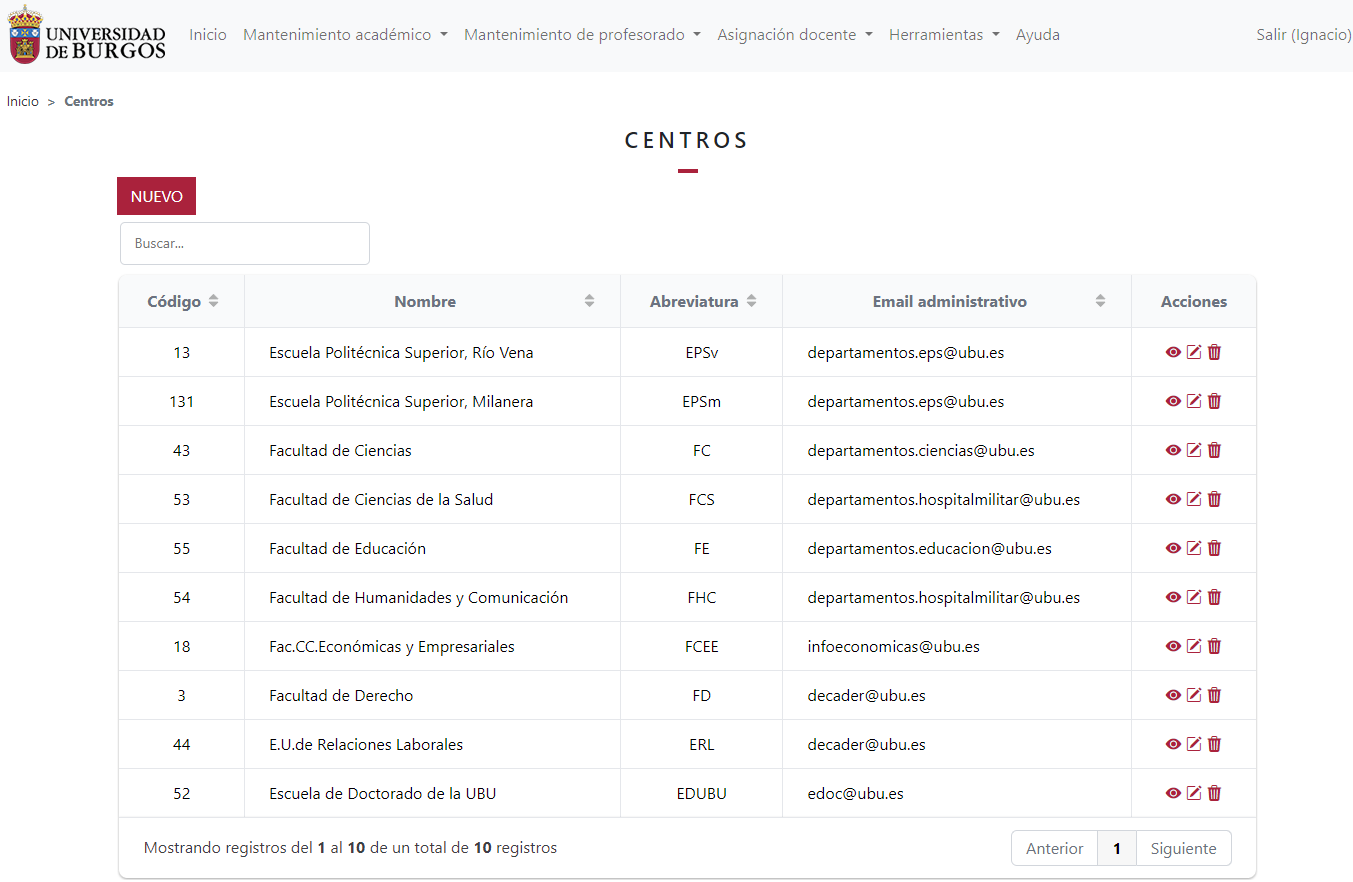
\includegraphics[width=\textwidth]{../img/Anexos/Manual usuario/centros.png}
	\caption{Página principal de centros}\label{pag:centros}
\end{figure}

\begin{figure}
	\centering
	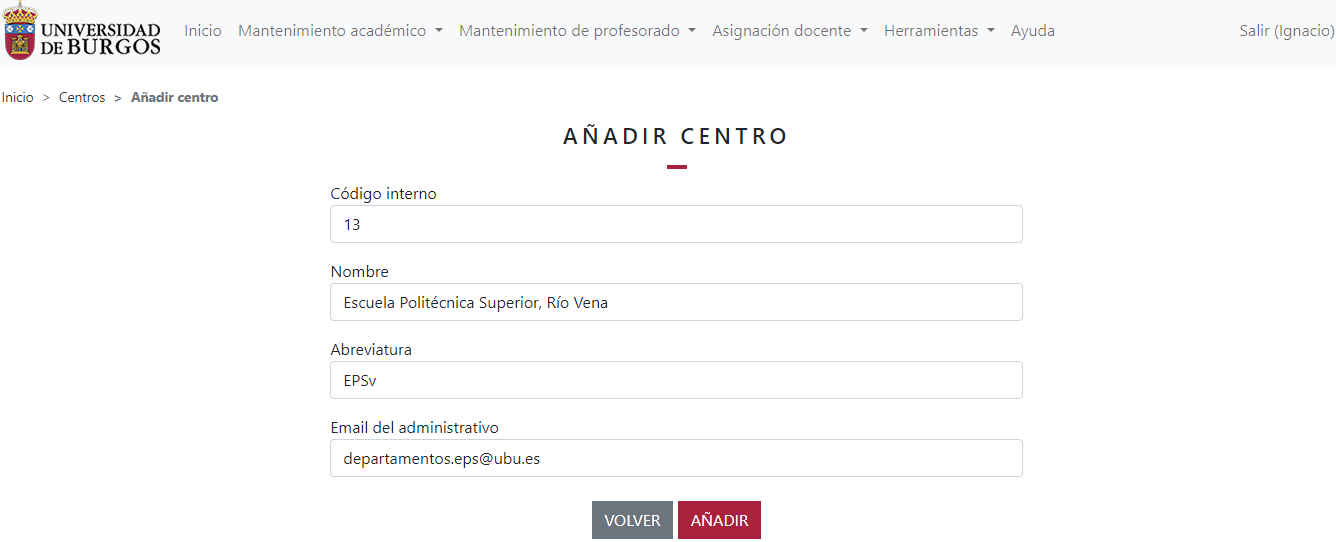
\includegraphics[width=\textwidth]{../img/Anexos/Manual usuario/formCentro.png}
	\caption{Formulario de creación de centros}\label{pag:formCentro}
\end{figure}

Desde la página del formulario se deben rellenar los campos con los datos del nuevo centro y pulsar sobre el botón <<Añadir>>.
Esto provocará que el centro se almacene en la base de datos. 
La aplicación redirigirá al usuario a la página principal de centros (imagen~\ref{pag:centros}) mostrando un mensaje que indica la correcta creación del centro.

\subsubsection{Modificación de centros}
Desde la página principal de centros (imagen~\ref{pag:centros}), se debe pulsar, en la tabla, sobre el icono del lápiz del centro que se desea modificar.
Esta acción provocará la redirección a la página del formulario de modificación, que contendrá los datos del centro seleccionado (imagen~\ref{pag:formModCentro}).

Desde esta página se pueden modificar los campos deseados y, al finalizar, pulsar sobre el botón <<Modificar>>.
Esta acción producirá una redirección a la página principal de centros, mostrando un mensaje que indica la correcta modificación del centro.

\begin{figure}
	\centering
	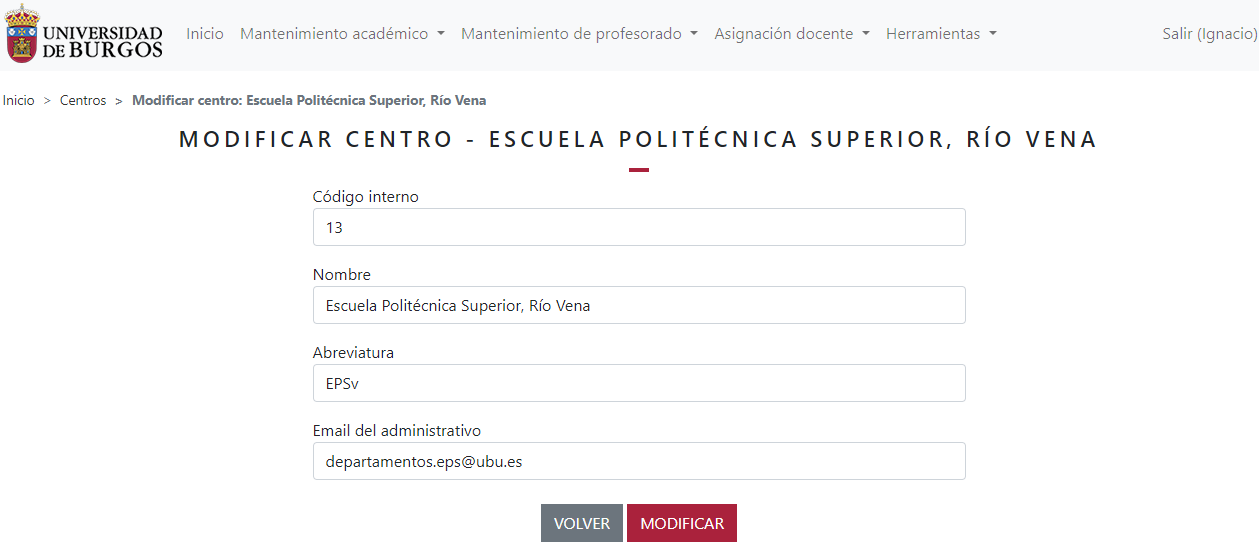
\includegraphics[width=\textwidth]{../img/Anexos/Manual usuario/formModCentro.png}
	\caption{Formulario de modificación de centros}\label{pag:formModCentro}
\end{figure}

\subsubsection{Eliminación de centros}
Desde la página principal de centros se puede eliminar un centro pulsando sobre el icono de la papelera del centro de la tabla que se desea eliminar.
Al hacer esto se mostrará la alerta de la imagen~\ref{pag:alertElCentro} y pulsando sobre el botón <<Aceptar>>, se realizará la petición de eliminación del centro.

Al hacer esto se mostrará un mensaje indicando la correcta eliminación o un mensaje indicando que no se ha podido realizar la eliminación en caso de que el centro tenga titulaciones asociadas.

\begin{figure}
	\centering
	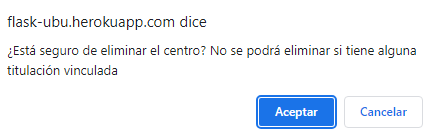
\includegraphics[width=\textwidth]{../img/Anexos/Manual usuario/alertElCentro.png}
	\caption{Alerta de eliminación de centros}\label{pag:alertElCentro}
\end{figure}

\subsubsection{Creación de titulaciones}
Pulsando sobre la opción del menú <<Titulaciones>> se accede a la vista principal de las titulaciones (ver imagen~\ref{pag:titulaciones}).

Para crear una nueva titulación se debe pulsar sobre el botón <<Nuevo>>.
Es importante tener en cuenta que para crear una titulación es necesario tener un centro creado previamente, ya que una titulación se vincula a un centro.

\begin{figure}
	\centering
	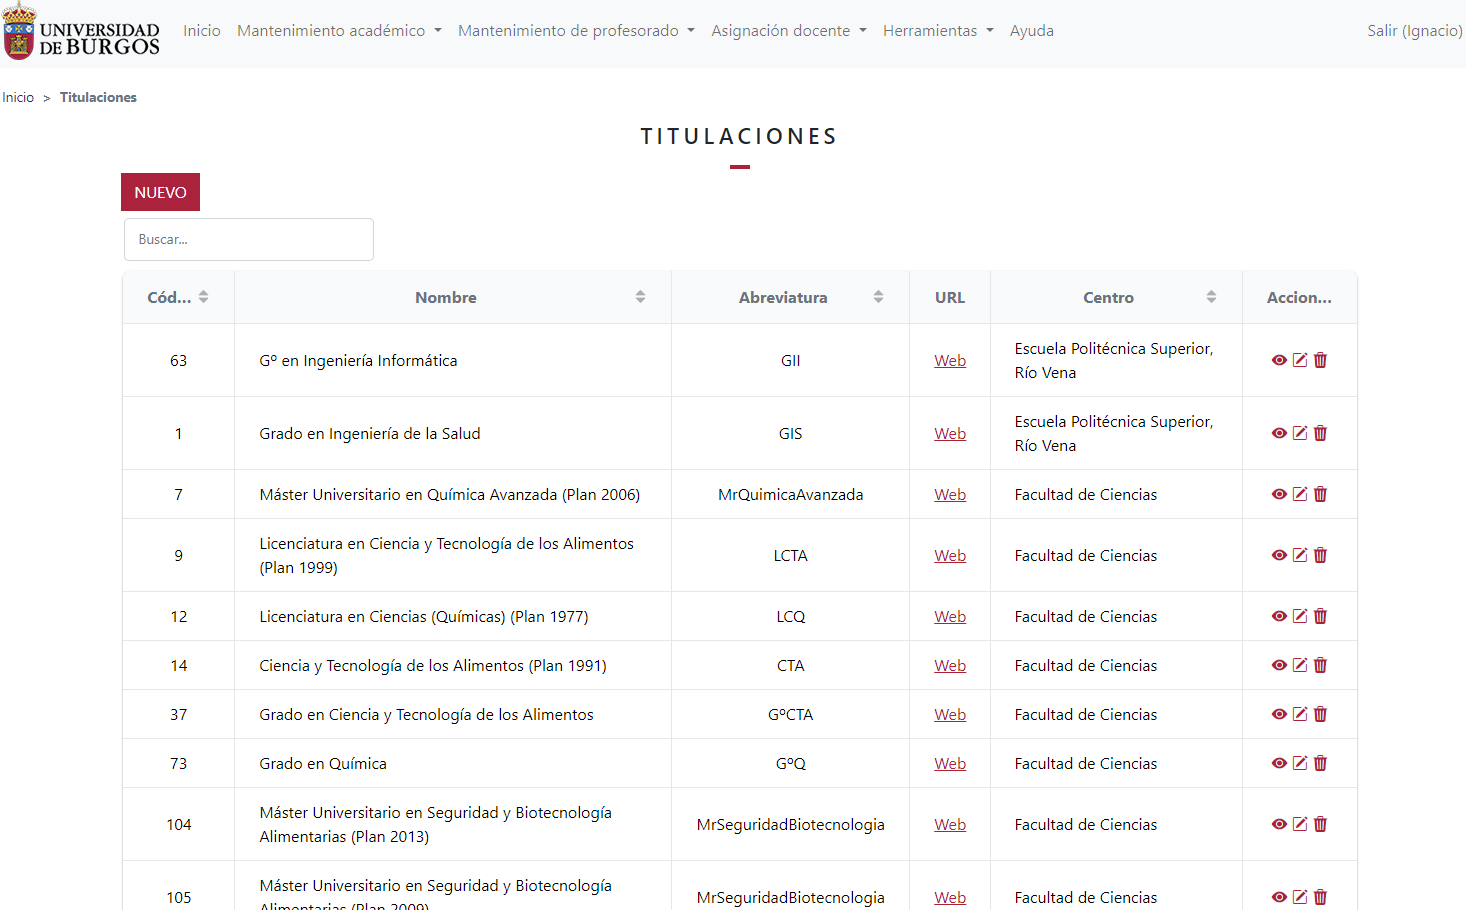
\includegraphics[width=\textwidth]{../img/Anexos/Manual usuario/titulaciones.png}
	\caption{Página principal de titulaciones}\label{pag:titulaciones}
\end{figure}

Al pulsar sobre el botón <<Nuevo>> se abre el formulario de creación de titulaciones.
Está página se puede ver en la imagen~\ref{pag:formTitulacion}.
En este formulario se deben introducir los datos de la titulación que se desea crear y, una vez se tengan los campos completados, pulsar sobre el botón <<Añadir>>.
Esta acción producirá una redirección a la página principal de titulaciones donde se podrá ver la titulación creada.
Además, se mostrará un mensaje indicando la creación de la titulación.

\begin{figure}
	\centering
	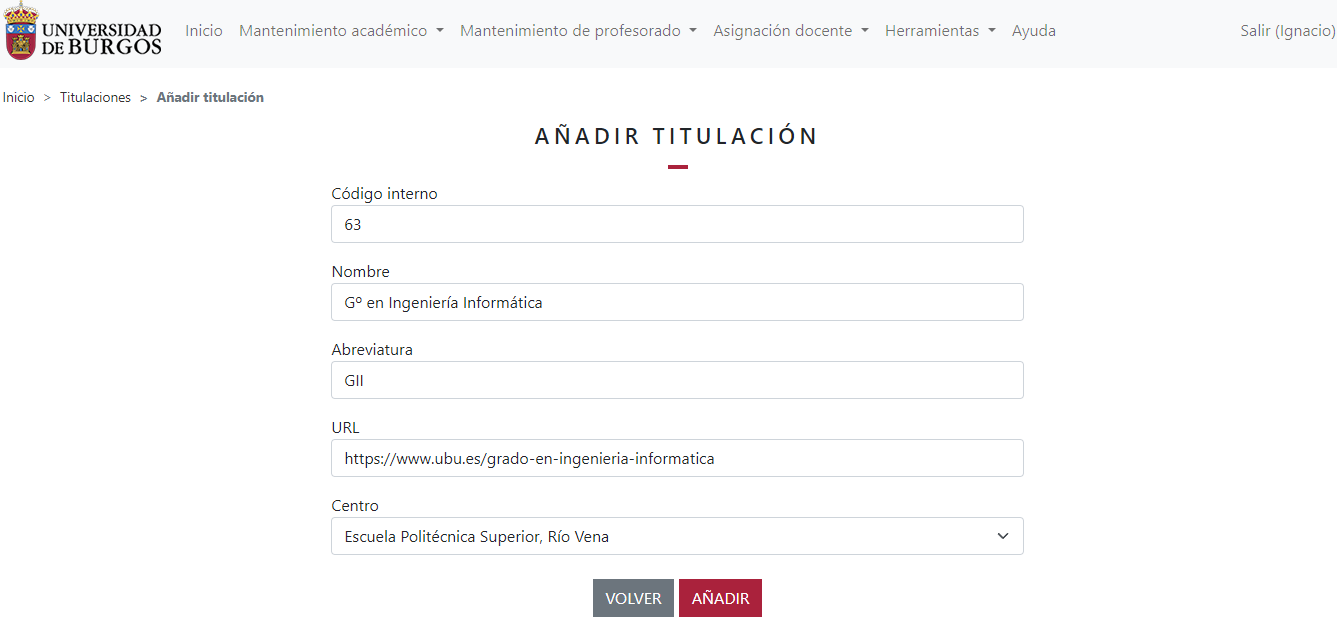
\includegraphics[width=\textwidth]{../img/Anexos/Manual usuario/formTitulacion.png}
	\caption{Formulario de creación de titulaciones}\label{pag:formTitulacion}
\end{figure}

\subsubsection{Modificación de titulaciones}
Para modificar una titulación, encontrándonos en la página principal de titulaciones (imagen~\ref{pag:titulaciones}), se debe pulsar sobre el icono de la lápiz de la titulación de la lista que se desea modificar.
Esto abrirá la página con el formulario de modificación de la titulación (ver imagen~\ref{pag:formModTitulacion}).

\begin{figure}
	\centering
	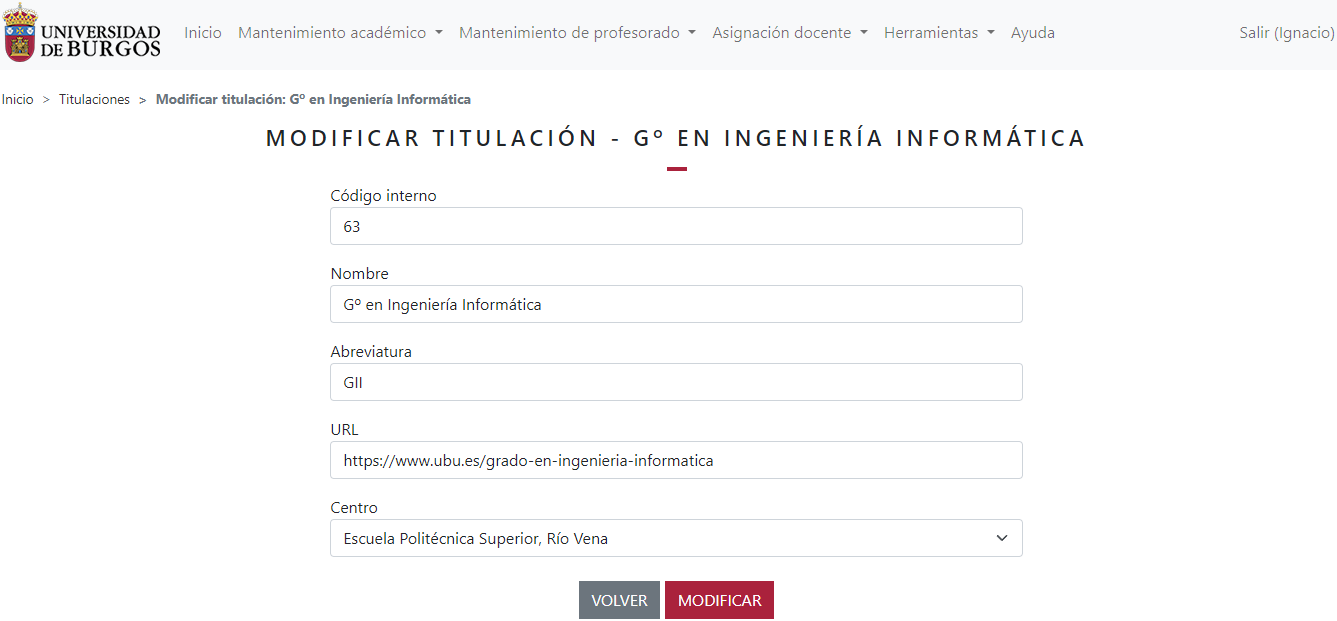
\includegraphics[width=\textwidth]{../img/Anexos/Manual usuario/formModTitulacion.png}
	\caption{Formulario de modificación de titulaciones}\label{pag:formModTitulacion}
\end{figure}

Desde este formulario se pueden modificar los campos deseados.
Una vez concluida la modificación se debe pulsar sobre el botón <<Modificar>>.
Esto plasmará los cambios en la base de datos y la web redirigirá al usuario a la página principal de titulaciones indicando mediante un mensaje la correcta modificación.

\subsubsection{Eliminación de titulaciones}
Desde la página principal de titulaciones (imagen~\ref{pag:titulaciones}), se debe pulsar sobre el icono de la papelera de la titulación que se desea eliminar.
Al realizar esta acción aparecerá en la pantalla la alerta de la imagen~\ref{pag:alertElTitulacion}. Si se pulsa sobre el botón <<Aceptar>> la titulación se eliminará de la base de datos si no tiene asignaturas asociadas, en caso contrario, no se podrá eliminar y aparecerá un mensaje de error mostrando esta información.

\begin{figure}
	\centering
	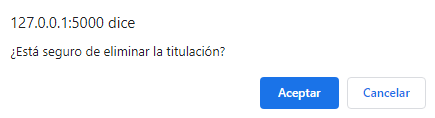
\includegraphics[width=\textwidth]{../img/Anexos/Manual usuario/alertElTitulacion.png}
	\caption{Alerta de eliminación de titulaciones}\label{pag:alertElTitulacion}
\end{figure}

\subsubsection{Creación de asignaturas}
Para añadir una nueva asignatura a la web, se debe pulsar sobre la opción del menú llamada <<Asignaturas>>.
Realizar esta acción redirige al usuario a la página principal de asignaturas (imagen~\ref{pag:asignaturas}).

Es importante tener en cuenta que previamente se debe haber creado la titulación a la que se quiere vincular la asignatura.

\begin{figure}
	\centering
	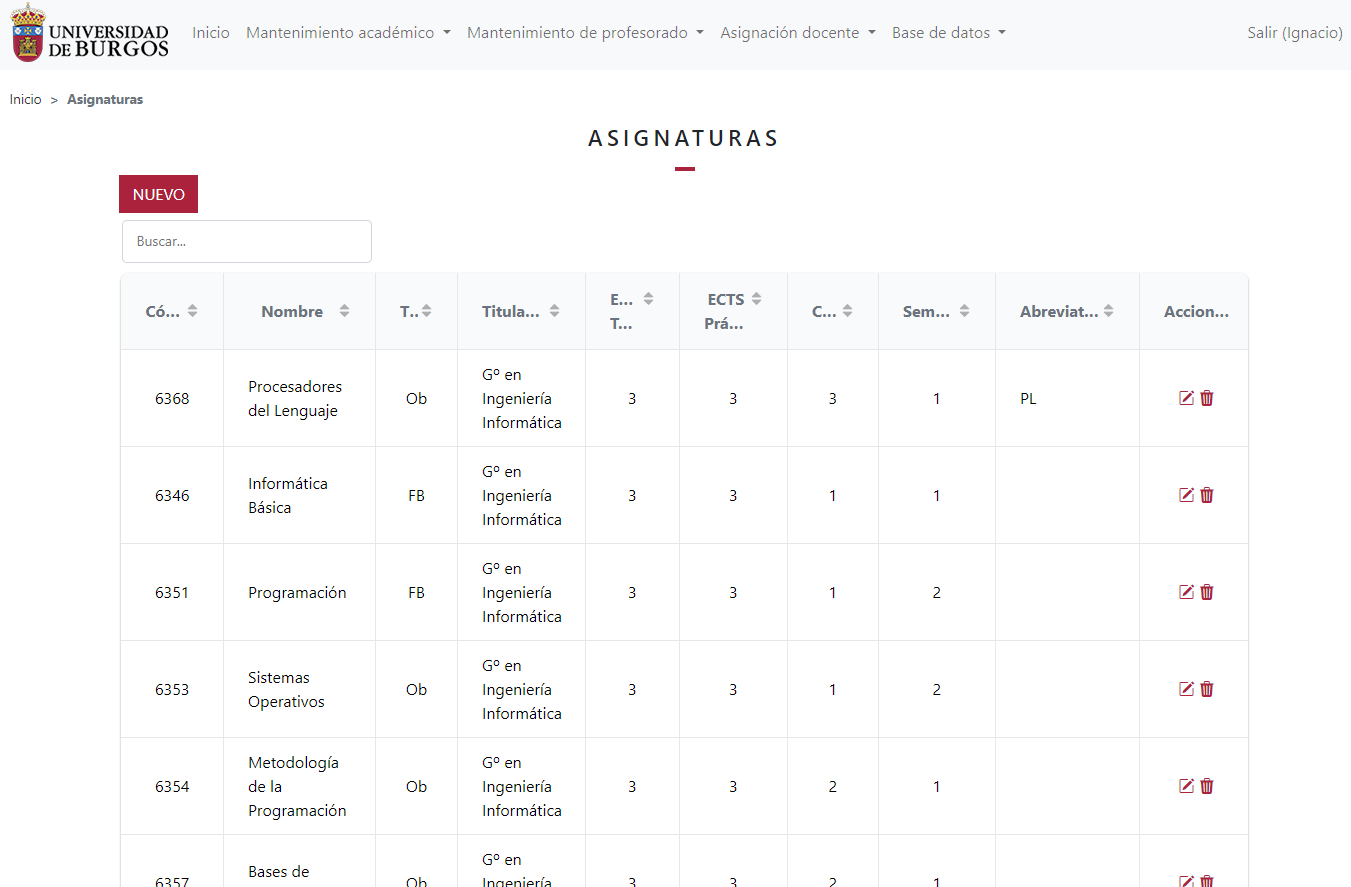
\includegraphics[width=\textwidth]{../img/Anexos/Manual usuario/asignaturas.png}
	\caption{Página principal de asignaturas}\label{pag:asignaturas}
\end{figure}

Una vez en la página principal de asignaturas se debe pulsar sobre el botón <<Nuevo>>, lo que abrirá el formulario de creación de asignaturas (ver imagen~\ref{pag:formAsignatura}).

Con los campos del formulario completados solo queda pulsar sobre el botón <<Añadir>> para almacenar la asignatura en la base de datos.
Tras realizar esta acción, se mostrará la página principal de asignaturas junto a un mensaje informando de la correcta creación de la asignatura.

\begin{figure}
	\centering
	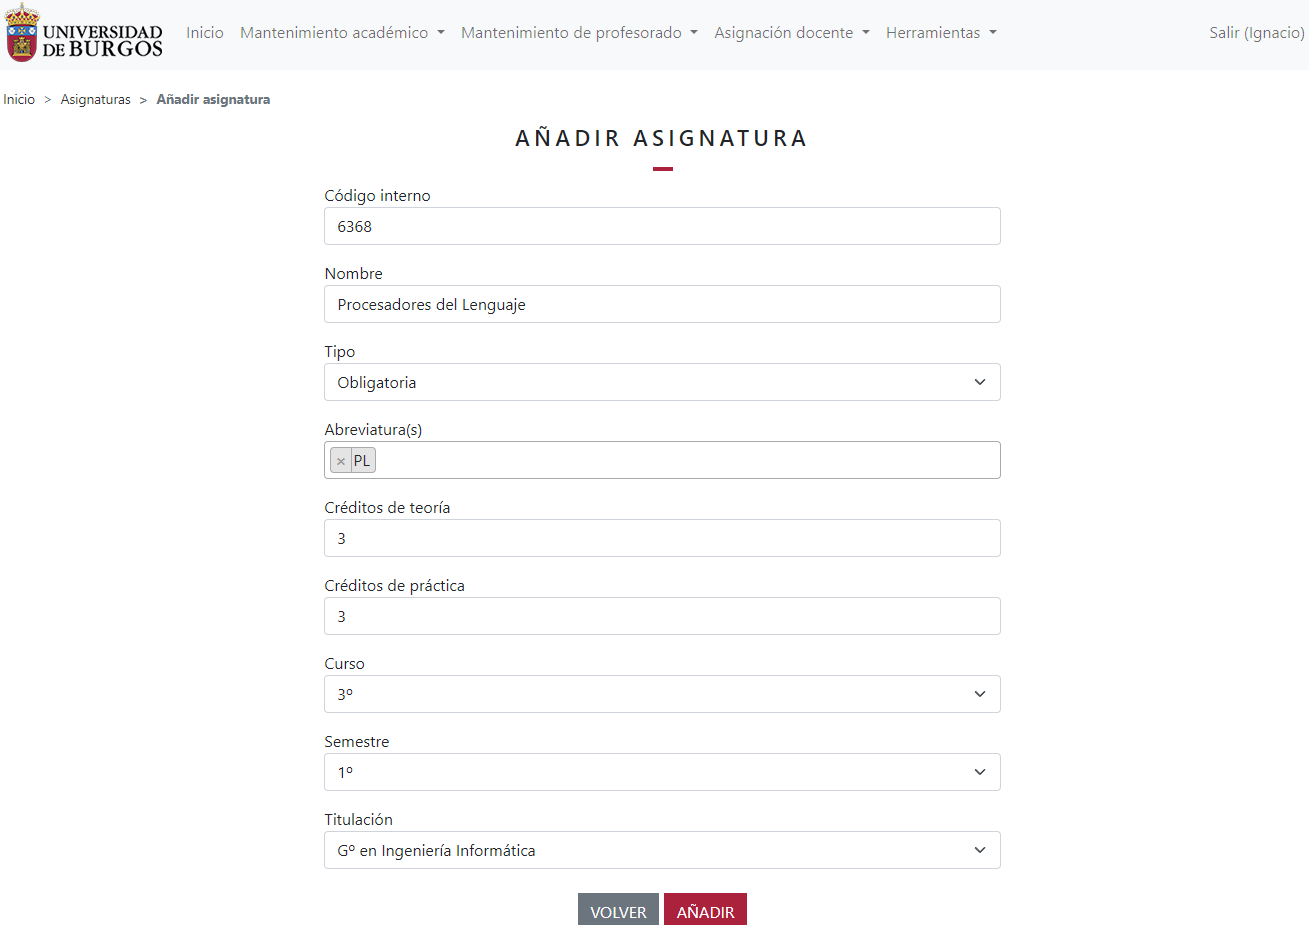
\includegraphics[width=\textwidth]{../img/Anexos/Manual usuario/formAsignatura.png}
	\caption{Formulario de creación de asignaturas}\label{pag:formAsignatura}
\end{figure}

\subsubsection{Modificación de asignaturas}
Para modificar una asignatura se debe pulsar sobre el icono del lápiz de la asignatura de la tabla que se desea modificar.
Esto abrirá el formulario de modificación de la asignatura con los campo rellenos con la información de la asignatura a editar (ver imagen~\ref{pag:formModAsignatura}).

En este momento se pueden editar los campos deseados y al finalizar, se debe pulsar sobre el botón <<Modificar>>.
Esto provocará el guardado de la información y una redirección a la página de asignaturas donde se mostrará un mensaje informativo sobre la modificación de la asignatura.

\begin{figure}
	\centering
	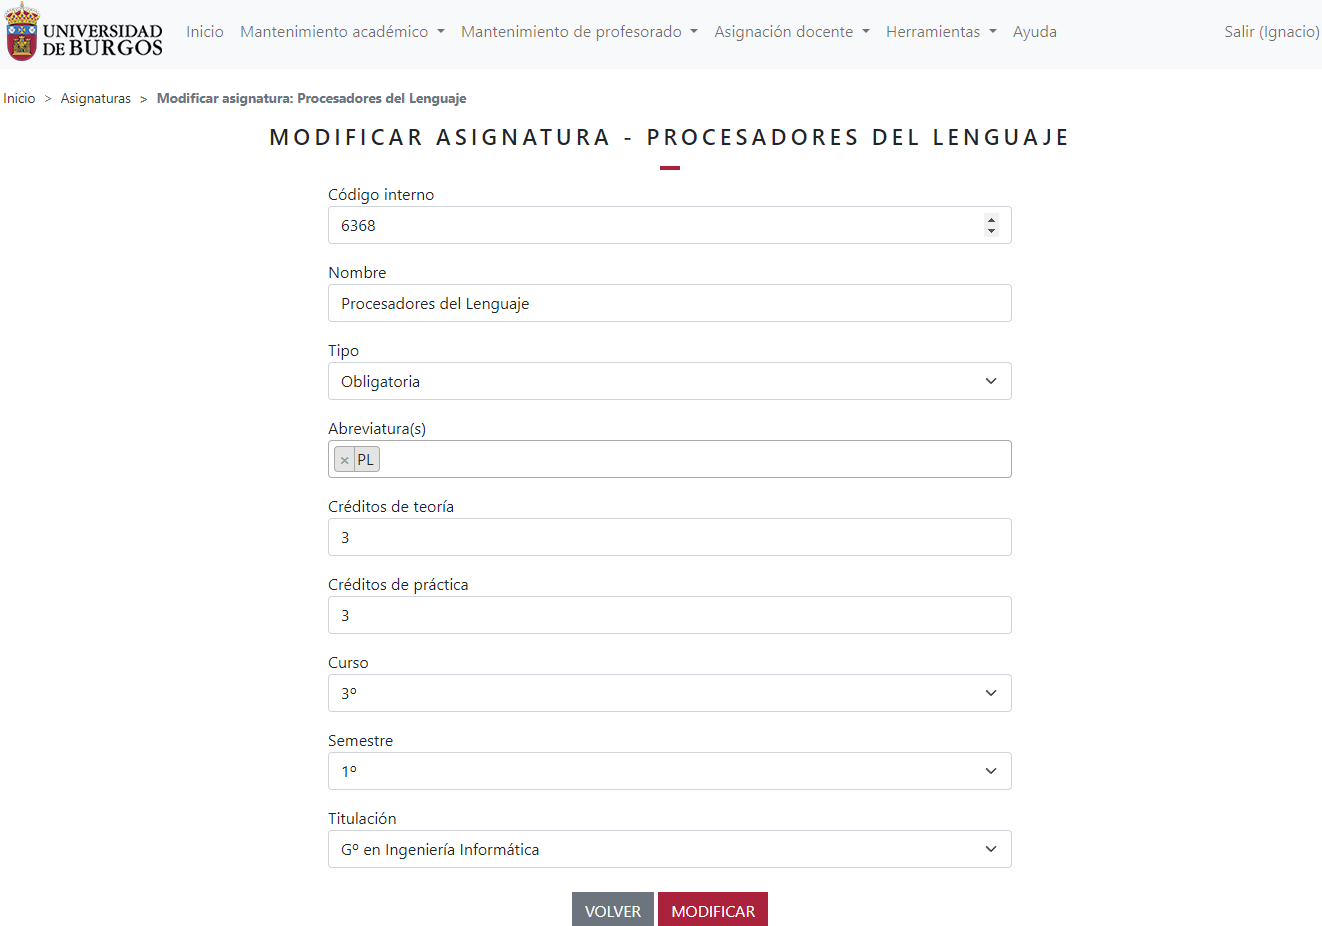
\includegraphics[width=\textwidth]{../img/Anexos/Manual usuario/formModAsignatura.png}
	\caption{Formulario de modificación de asignaturas}\label{pag:formModAsignatura}
\end{figure}

\subsubsection{Eliminación de asignaturas}
Si se desea eliminar una asignatura de la aplicación, se debe acceder a la página principal de asignaturas y, una vez aquí, pulsar sobre el icono de la papelera de la asignatura que se desea eliminar.

Al realizar la acción descrita, se abre una alerta de confirmación (ver imagen~\ref{pag:alertElAsignatura}).
Al pulsar sobre <<Aceptar>> la asignatura se elimina de la aplicación produciendo un borrado en cascada de sus relaciones con los cursos académicos creados.

\begin{figure}
	\centering
	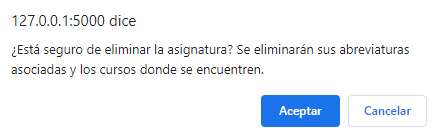
\includegraphics[width=.8\textwidth]{../img/Anexos/Manual usuario/alertElAsignatura.png}
	\caption{Alerta de eliminación de titulaciones}\label{pag:alertElAsignatura}
\end{figure}

\subsection{Mantenimiento de profesorado}
En esta sección se va a mostrar el manual de usuario sobre el mantenimiento de profesorado.
Esta parte de la aplicación incluye la creación, modificación y eliminación de los elementos que se pueden ver en la imagen~\ref{pag:menuManProf}.

\begin{figure}
	\centering
	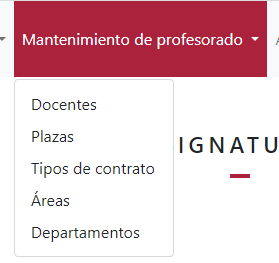
\includegraphics[width=.5\textwidth]{../img/Anexos/Manual usuario/menu man prof.png}
	\caption{Menú: Mantenimiento de profesorado}\label{pag:menuManProf}
\end{figure}

\subsubsection{Creación de docentes}

\subsubsection{Modificación de docentes}

\subsubsection{Eliminación de docentes}


\subsubsection{Creación de plazas}

\subsubsection{Modificación de plazas}

\subsubsection{Eliminación de plazas}


\subsubsection{Creación de tipos de contrato}

\subsubsection{Modificación de tipos de contrato}

\subsubsection{Eliminación de tipos de contrato}


\subsubsection{Creación de áreas}

\subsubsection{Modificación de áreas}

\subsubsection{Eliminación de áreas}


\subsubsection{Creación de departamentos}

\subsubsection{Modificación de departamentos}

\subsubsection{Eliminación de departamentos}
